O Diagrama Entidade-Relacionamento da Figura~\ref{fig:der} modela a estrutura do banco de dados implementada no MVP do sistema, composta por duas entidades principais: \code{CERTIFICADOS} e \code{TEMPLATES}. A notação adotada é a pé-de-galinha (Engenharia da Informação), onde o símbolo de barra (---) indica o lado ``1'' e o símbolo de três pontas (--<) indica o lado ``N'' (muitos). Ambas as entidades utilizam UUID como identificador primário.

A entidade \code{CERTIFICADOS} armazena os certificados emitidos e contém os seguintes atributos: \code{id} (PK, UUID), \code{recipientName} (varchar 200, NOT NULL), \code{recipientCPF} (varchar 11, NOT NULL, indexado), \code{courseName} (varchar 300, NOT NULL), \code{courseHours} (integer, NOT NULL), \code{verificationCode} (varchar 8, UNIQUE, NOT NULL), \code{validityDate} (timestamptz, NOT NULL), \code{templateId} (FK, UUID, NOT NULL), \code{issuedAt} (timestamptz, NOT NULL), \code{createdAt} (timestamptz, NOT NULL) e \code{updatedAt} (timestamptz, NOT NULL).

A entidade \code{TEMPLATES} gerencia os modelos de certificado disponíveis para emissão, com os atributos: \code{id} (PK, UUID), \code{name} (varchar 100, NOT NULL), \code{description} (text), \code{layoutConfig} (jsonb), \code{createdAt} (timestamptz, NOT NULL) e \code{updatedAt} (timestamptz, NOT NULL).

O relacionamento entre as entidades é de 1:N (um template pode ser usado por vários certificados), materializado pela chave estrangeira \code{templateId} na entidade \code{CERTIFICADOS} que referencia \code{TEMPLATES(id)}. Essa modelagem reflete o escopo reduzido do MVP, que contempla exclusivamente as funcionalidades de emissão de certificados com suporte a templates personalizáveis, sem as entidades de usuários, organizações, participantes, cursos e auditoria que serão incorporadas em versões futuras do sistema.

Vale ressaltar que, no estado atual do sistema, as informações relativas a participantes e cursos são armazenadas de forma denormalizada diretamente na entidade \code{CERTIFICADOS}, por meio dos atributos \code{recipientName}, \code{recipientCPF}, \code{courseName} e \code{courseHours}. Essa abordagem elimina a necessidade de chaves estrangeiras para entidades de participantes e cursos, simplificando a implementação do MVP, porém introduz redundância de dados e compromete a integridade referencial. Em versões futuras, as entidades \code{PARTICIPANTES} e \code{CURSOS} serão materializadas no banco de dados, permitindo a associação por meio de chaves estrangeiras (\code{participantId} e \code{courseId}), eliminando a duplicação de dados e habilitando funcionalidades como histórico de certificados por participante, listagem de certificados por curso e relatórios gerenciais por unidade de treinamento.

O Diagrama de Classes (Figura~\ref{fig:diagrama-classes}) apresenta a hierarquia \code{PESSOA} $\rightarrow$ \code{USUARIO} / \code{PARTICIPANTE} como uma generalização conceitual oriunda do modelo de domínio. No banco de dados físico do MVP, essas entidades não foram materializadas --- apenas \code{CERTIFICADOS} e \code{TEMPLATES} existem como tabelas. A implementação futura dessa herança seguirá a estratégia \textit{joined-table} (ou \textit{table-per-type}), na qual \code{PESSOA} seria uma tabela concreta com os atributos comuns (\code{id}, \code{nome}, \code{email}) e cada subtipo (\code{USUARIO}, \code{PARTICIPANTE}) teria sua própria tabela com chave primária que é também chave estrangeira referenciando \code{PESSOA(id)} --- garantindo integridade referencial sem armazenamento redundante.

\begin{figure}[H]
    \centering
    \caption{Diagrama Entidade-Relacionamento (DER) --- MVP do Banco de Dados}
    \label{fig:der}
    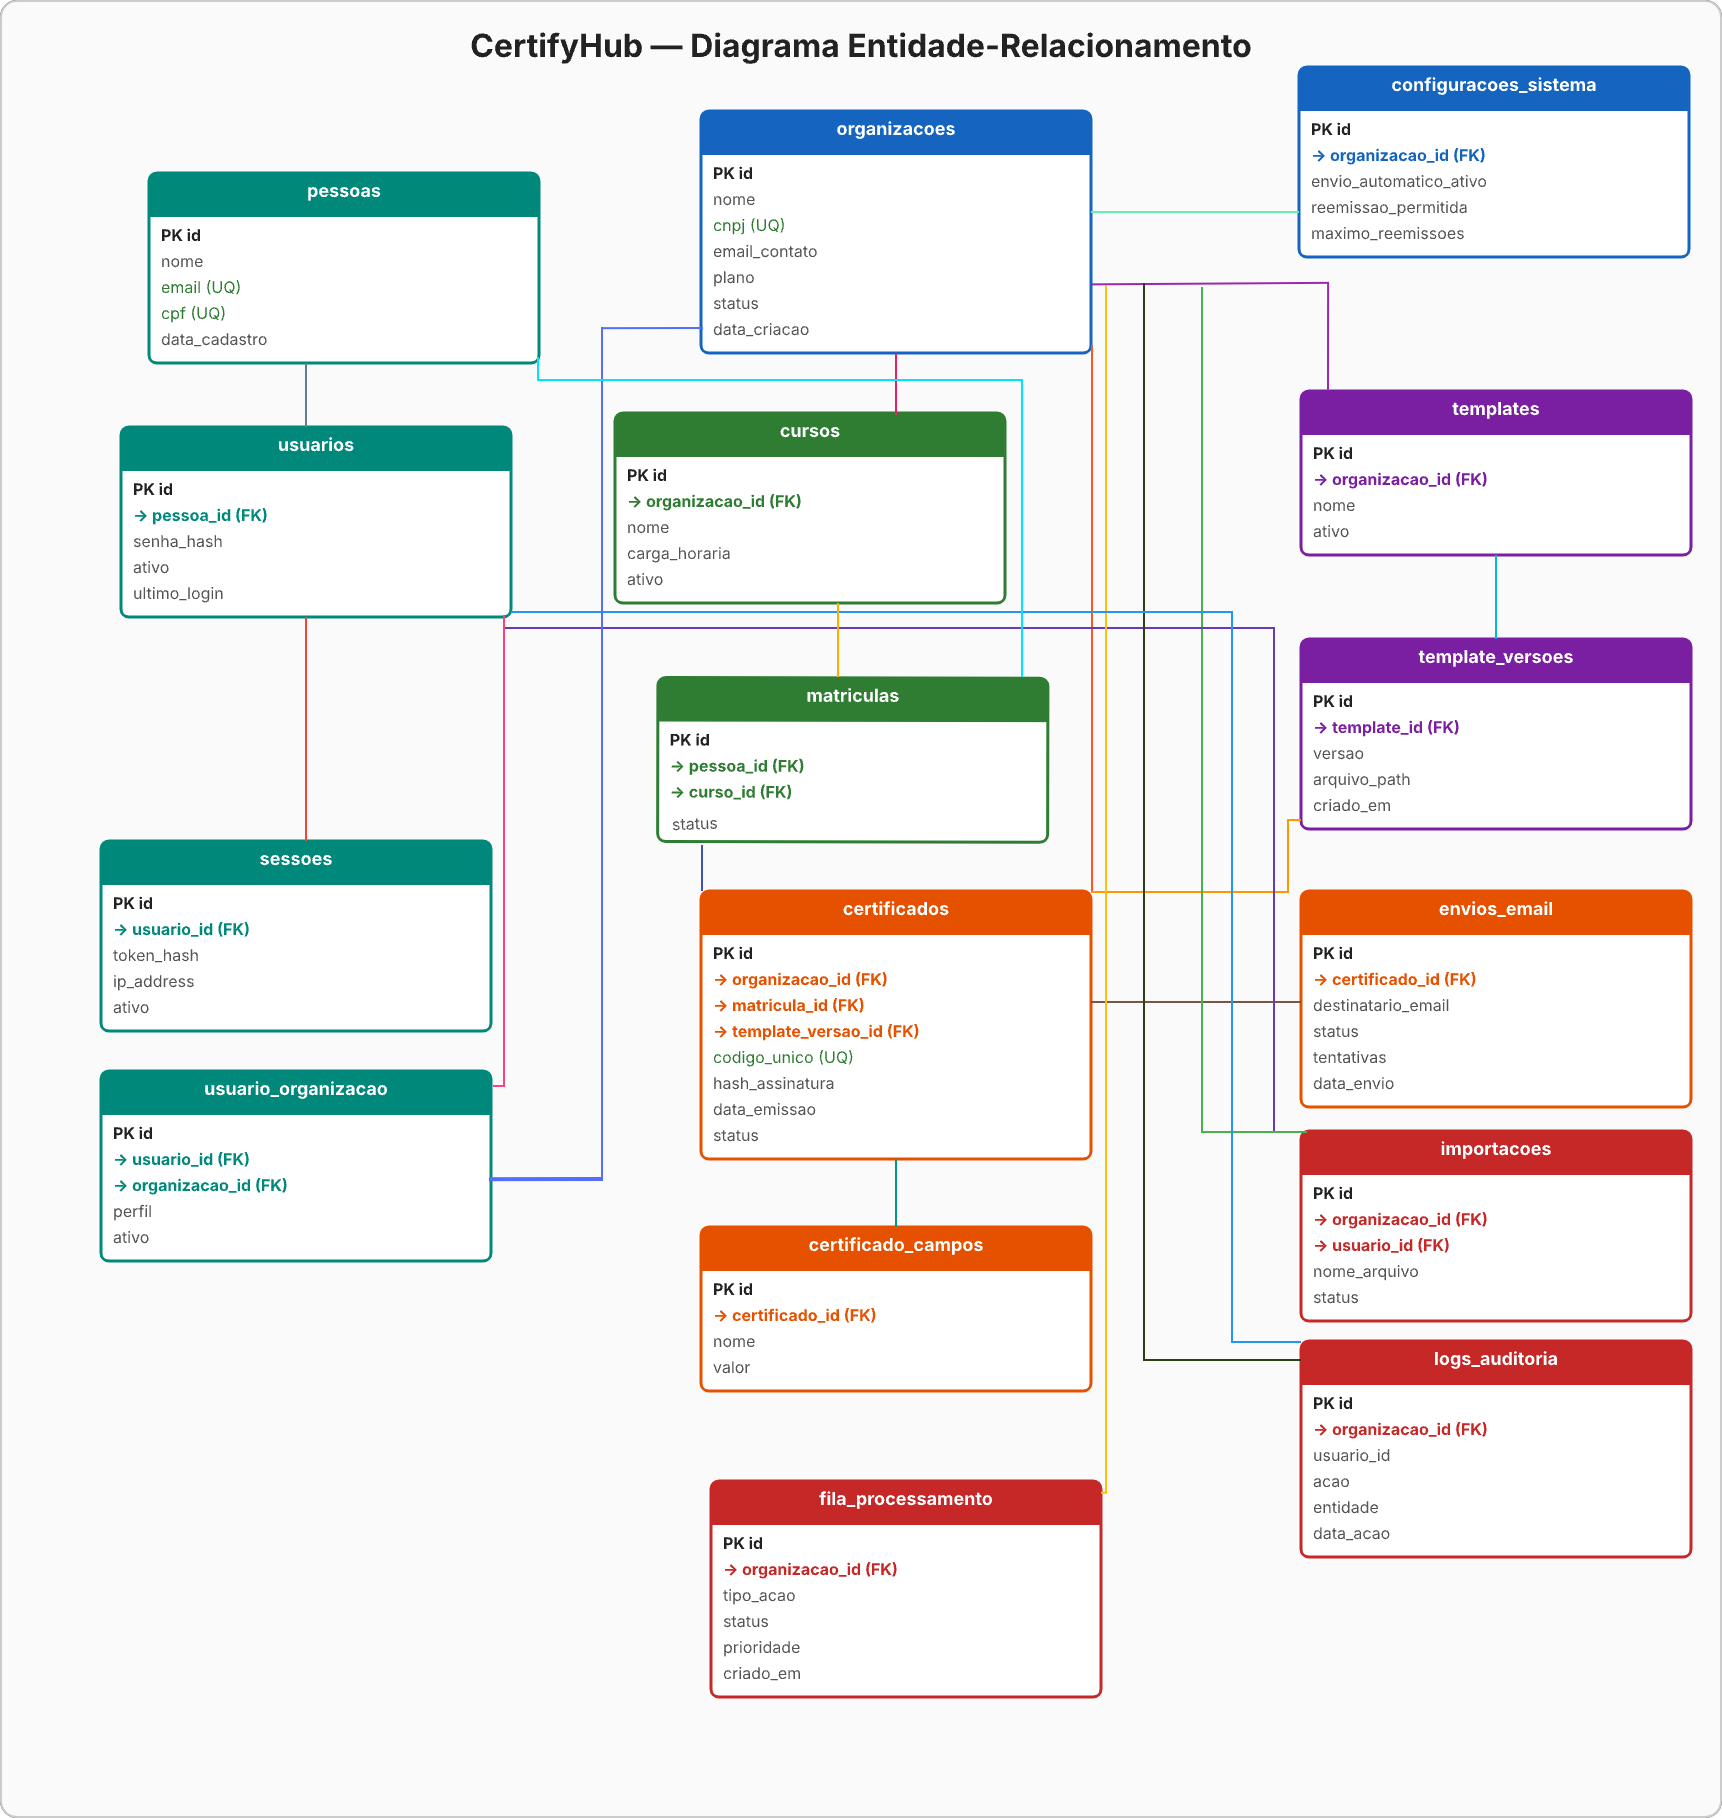
\includegraphics[width=0.9\textwidth]{imagens/DER.png}
\end{figure}
